\subsection{Cloud-To-Thing Kontinuum} % (fold)
\label{sub:Cloud-To-Thing-Continuum}

Das \acrlong{cttc} beschreibt die Möglichkeit zur Nutzung von Speicher und Rechenkapazitäten, sowie der Sammlung von Daten auf einem Kontinuum. Das Kontinuum enthält, wie in \cite{cominardiDevopsEdgeopsVision2021} beschrieben, verschiedene Arten von Ressourcen die sich in mehreren Netzwerken oder geographischen Orten befinden. Die Ressourcen reichen von Roboter, über Edge Server bis hin zu Cloud Instanzen.

\begin{figure}
  \begin{center}
    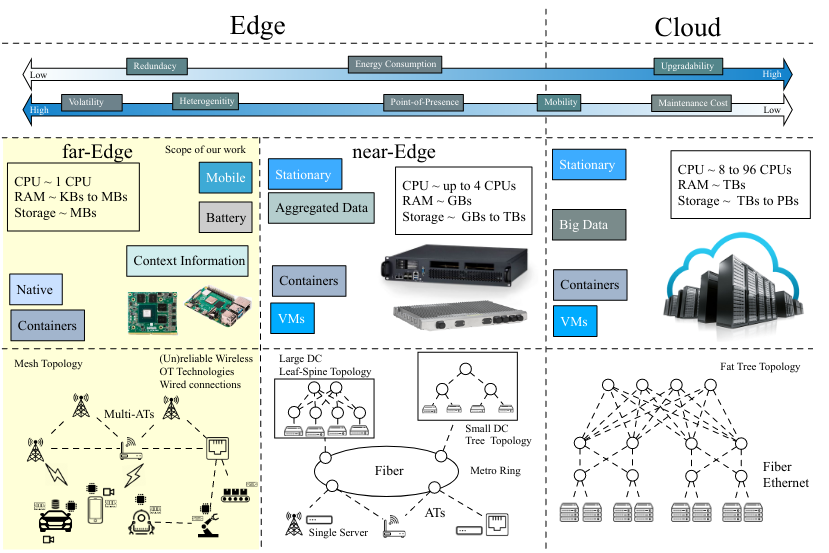
\includegraphics[width=0.95\textwidth]{./figures/cloud-thing-continuum.png}
  \end{center}
  \caption{Übersicht \acrlong{cttc} \cite{baldoniManagingFarEdgeAre2021}}
  \label{fig:cttc}
\end{figure}

Wie man in der Grafik \ref{fig:cttc} erkennen kann, hat man unterschiedliche heterogene Ressourcen die verschiedene Eigenschaften haben und unter verschiedenen Bedingungen agieren. Auf der einen Seite, hat man am Edge ein sehr heterogenes System mit Beispielsweise Robotern und IoT Geräten. Diese besitzen eingeschränkte Ressourcen wie Beispielsweise Rechenkapazitäten. Hinzu kommen unverlässliche Verbindungen wie Wi-Fi oder Bluetooth.\\
Auf der anderen Seite, befinden sich die Cloud Instanzen. Dessen Ressourcen sind recht homogen und verlässlich. Größtenteils also das genaue Gegenteil zu den Geräten nahe dem Edge. Zwischen den beiden Schichten befinden sich oftmals Edge Server. Diese ähneln den Komponenten der Cloud. Da sie aber von der Lokalität nahe an den Endgeräten sein müssen, sind Sie nicht so einfach Skalierbar wie Cloud Ressourcen.\\
Aufgrund der unterschiedlichen Gegebenheiten und Eigenschaften der Geräte, ist es wichtig ein einheitliches Kommunikationsmedium zu nutzen welches die Komponenten der verschiedenen Schichten unterstützt. Im Bereich der Robotik, wurden diese Aspekte ende 2018 in \cite{jawharNetworkingMultiRobotSystems2018} untersucht. Im Artikel wurde das \acrlong{cttc} als R2I(robot-to-infrastructure) beschrieben. Dabei wurden MRS(Multi-Robot-Systems) und die Möglichkeiten der Kommunikation verglichen. Beim Vergleich kamen die Autoren zu einer Ähnlichen Schlussfolgerung wie eingangs erwähnt: "This gateway node must be able to map the networking parameters associated with the data traffic in the data link layer header to the corresponding data link layer header in the infrastructure network." \cite{jawharNetworkingMultiRobotSystems2018}. Gemeint, sind die verschiedenen Protokolle die unterstützt werden müssen um sowohl Robotik als auch weitere Infrastruktur Systeme miteinander zu verbinden. Das Paper beschreibt zudem Grundprotokolle wie Wi-Fi oder Bluetooth die zum Austausch der Nachrichten benötigt werden. Wie man an den zahlreichen im Paper genannten Technologien erkennen kann, ist der Bereich um die Kommunikation im Robot to Infrastructure Bereich sehr Komplex. Das \acrlong{cttc} zielt dabei auf eine Vereinheitlichung der Kommunikationswege aus. Dabei wird eine Technologie gesucht, die bereits bestehende Protokolle unterstützt, abstrahiert oder ersetzt und als Ende zu Ende Lösung genutzt werden kann. Im folgenden Teil dieser Arbeit wird sich dieser Frage gewidmet.
